\section{Interazione tra le Entità}

Viene ora presentata una descrizione delle interazioni tra le varie entità introdotte nella sezione precedente. La progettazione delle entità reattive viene descritta mediante il costrutto \ii{monitor} presentato a lezione, supponendo quindi di avere una struttura dati che incapsula la risorsa esponendo procedure accessibili in mutua esclusione dai thread; inoltre si suppone l'esistenza dei costrutti \ttt{wait(var\_condizione)} e \ttt{signal(var\_condizione)}, i quali rispettivamente forzano l'attesa del chiamante su coda FIFO, e risvegliano il primo processo in attesa su tale coda. Si suppone inoltre la presenza di un costrutto \ttt{signal\_all(val\_condizione)} il quale risveglia ordinatamente tutti i thread in attesa su una data variabile di condizione.

\subsection{Percorrenza di un Viaggiatore}\label{subsec:percorrenza_viaggiatore}
	
	Alla luce della definizione dell'entità Viaggiatore in sezione \ref{subsec:traveler_def}, è possibile definire le azioni che compongono il viaggio:
		\begin{itemize}
			\item Acquisto di un Biglietto (\ttt{Ticket}) presso la Biglietteria della Stazione (\ttt{Ticket\_Office}) di partenza. Ogni Biglietto è composto da una sequenza ordinata di Tappe (\ttt{Ticket\_Stages}), ciascuna contenente:
				\begin{verbatim}
					- start_station
					- next_station
					- train_id 
					- start_platform 
					- destination_platform
					- run_number
					- next_region
				\end{verbatim}
			e da un indice della prossima tappa del Percorso (\ttt{Next\_Stage}). Nel caso in cui il Treno \ttt{train\_id} sia un Treno a prenotazione, il valore di \ttt{run\_number} sarà $>$ 0.
			
			\item Una volta ottenuto un Ticket, vengono eseguite le seguenti operazioni per ciascuna Tappa del Biglietto:
				\begin{itemize}
					\item Accodamento presso la Piattaforma \ttt{start\_platform} della Stazione \ttt{start\_station} in attesa del Treno \ttt{train\_id}.
					\item All'arrivo del treno \ttt{train\_id}, Accodamento presso la Piattaforma \ttt{destination\_platform} della Stazione \ttt{next\_station} in attesa dell'arrivo di \ttt{train\_id}. 
				\end{itemize}
		\end{itemize} 
	Le azioni sopraelencate possono essere incapsulate in strutture dati che rappresentano una specifica operazione. In questo modo viene generata una \ii{gerarchia di operazioni}, tutte derivanti da un'unica \ii{operazione generica}. Di seguito identificheremo tali operazioni rispettivamente con \ttt{BUY\_TICKET}, \ttt{LEAVE} e \ttt{ARRIVE}.
	
	Il protocollo di operazioni che vengono eseguite da un Viaggiatore, è stato mantenuto il più semplice possibile, e l'intero percorso viene regolato dagli eventi generati dalle entità Treno alla partenza e all'arrivo dalle/nelle Stazioni. 
	
	\subsubsection{Acquisto di un Biglietto}\label{subsubsec:buy_ticket}
	
	L'acquisto di un Biglietto da parte di un Viaggiatore è effettuato tramite l'operazione \ttt{BUY\_TICKET}. Essa si limita a richiedere alla Biglietteria della Stazione di partenza (che viene definita da configurazione iniziale) un Biglietto per una specifica destinazione. Al termine della richiesta, l'esecuzione dell'operazione termina, e il thread corrente ritorna nella coda di thread \ttt{Traveler\_Pool} (descritta in sezione \ref{subsec:traveler_def}) per poter eseguire una nuova operazione. Questo comporta la definizione di una nuova operazione, \ttt{TICKET\_READY}, la quale verrà inserita nella coda di operazioni di \ttt{Traveler\_Pool}, all'avvenuta ricezione del Biglietto richiesto, sia per assegnare il \ttt{Ticket} creato e caricare nella coda della struttura dati \ttt{Traveler\_Pool} l'operazione \ttt{LEAVE} del Viaggiatore corrente, sia per eseguire operazioni in caso la richiesta non fosse andata a buon fine.
	
	\subsubsection{Partenza da una Stazione}
	
	Denominiamo $t$ la tappa di indice \ttt{Next\_Stage}, ovvero la tappa corrente. Perché l'operazione di Partenza dalla stazione corrente venga effettuata, è necessaria la precondizione per la quale:
	\begin{itemize}
		\item l'operazione \ttt{LEAVE} è stata inserita nella apposita coda di \ttt{Traveler\_Pool};
		\item in qualche momento essa venga prelevata (rimossa) da tale luogo ed eseguita da uno dei thread del pool di \ttt{Traveler\_Pool}. 
	\end{itemize}
Le azioni compiute dall'operazione \ttt{LEAVE} sono:
	
	\begin{itemize}
		\item Estrazione di \ttt{start\_station} da $t$;
		\item Tramite l'interfaccia esposta dalla Stazione \ttt{start\_station} (una procedura che identifichiamo con \ttt{Wait\_For\_Train\_To\_Go}), viene richiesto di attendere presso la Piattaforma \ttt{start\_platform}.
	\end{itemize} 
	
	Internamente alla Stazione, tale richiesta viene tradotta nell'inserimento del Viaggiatore, o meglio del suo Descrittore \ttt{Traveler\_Descriptor}, nella coda \ttt{Leaving\_Queue} della Piattaforma indicata da \ttt{start\_platform}. Tale operazione non utilizza una sezione critica presso la risorsa protetta a protezione della Piattaforma, ma possiamo pensare che la coda (FIFO) adottata sia ad accesso sincronizzato.
	
	Nel caso in cui la Stazione di partenza del Viaggiatore sia una Stazione di Gateway, allora la procedura di accodamento presso la Piattaforma designata diviene:
	\begin{itemize}
		\item Se la Regione di Destinazione \ttt{next\_region} è diversa dalla Regione corrente, allora
			\begin{itemize}
				\item I dati relativi al Viaggiatore (Descrittore e Biglietto) vengono serializzati (\ii{marshalling}).
				\item Viene inviato un messaggio alla prossima Regione (ovvero \ttt{next\_region}, il cui indirizzo viene recuperato dal Server dei Nomi) contente i dati serializzati, destinato alla Stazione di Gateway corrispondente in tale Regione (nodo).
				\item A destinazione, vengono aggiornati i dati relativi al Viaggiatore locale alla Regione e eseguito un accodamento presso la coda \ttt{Leaving\_Queue} della Piattaforma indicata da \ttt{start\_platform}.
			\end{itemize}
	\end{itemize}
	
	Il comportamento descritto non è proprio della operazione \ttt{LEAVE}, ma è contenuto nell'operazione della Piattaforma per l'accodamento del Viaggiatore presso la coda \ttt{Leaving\_Queue}. 
	
	
	\subsubsection{Arrivo alla Destinazione successiva}
		
	Similmente a quanto descritto per la partenza, l'arrivo a destinazione prevede che l'operazione \ttt{ARRIVE} sia già stata inserita all'interno della coda di operazioni in \ttt{Traveler\_Pool}, e che un thread del pool la esegua (rimuovendola dalla coda). A differenza della partenza, questa operazione può comportare l'accodamento del Viaggiatore presso una Stazione che non appartiene alla Regione (al nodo) corrente, anche se non di Gateway. 
	
	Vengono eseguite le seguenti azioni:
		\begin{itemize}
			\item Estrazione della prossima stazione (\ttt{next\_station}) e della Regione di destinazione (\ttt{next\_region}) dalla tappa corrente $t$. Si presentano ora due casi:
				\begin{itemize}
					\item Se la prossima Regione è la stessa della Regione corrente, allora mediante l'interfaccia esposta dalla Stazione locale \ttt{next\_station}, viene effettuata una richiesta di attesa presso la Piattaforma \\\ttt{destination\_platform}
					\item Se la destinazione è una Stazione appartenente ad un'altra Regione, allora:
						\begin{itemize}
							\item Viene individuato l'indirizzo della Regione remota (richiesto al \ttt{Name\_Server} che gestisce le Regioni).
							\item Vengono serializzati (\ii{marshalling}) i dati relativi al Viaggiatore (Descrittore del Viaggiatore) e al suo Biglietto.
							\item Viene inviato un Messaggio Remoto alla Regione specificata che provvederà ad effettuare l'aggiornamento del corrispondente Viaggiatore, e al suo accodamento presso la Stazione corretta.
						\end{itemize}
				\end{itemize}
		\end{itemize} 
		
	Internamente alla Stazione, la richiesta si traduce nell'inserimento del Descrittore del Viaggiatore corrente all'interno della coda \ttt{Arrival\_Queue} interna alla Piattaforma \ttt{destination\_platform} selezionata.
	
	Si noti che l'eventuale azione di trasferimento del Viaggiatore al nuovo nodo viene effettuata dall'operazione \ttt{ARRIVE} e non dalla stazione all'arrivo del Treno (descritto nella sottosezione \ref{subsubsec:regional_station_access}). Questa scelta è stata fatta per limitare il più possibile l'occupazione da parte di un Treno della Piattaforma (risorsa protetta), ed evitare quindi l'esecuzione di operazioni potenzialmente lunghe come l'invio di un messaggio remoto.

\newpage
	

	\subsection{Percorrenza di un Treno}
	
	A ciascuna entità Treno, è assegnato un Percorso (\ttt{Route}) che comprende andata e ritorno, composto da una sequenze di Tappe (\ttt{Stage}) successive, ciascuna contenente i seguenti campi:
				\begin{center}
\begin{verbatim}
    - start_station,
    - start_platform,
    - next_segment,
    - next_station,
    - next_platfom,
    - leave_action,
    - enter_action,
    - node_name
\end{verbatim}
				\end{center}
dove \ttt{leave\_action} e \ttt{enter\_action} indicano rispettivamente quello che un Treno dovrà compiere alla partenza dalla stazione \ttt{start\_station} e all'arrivo presso la prossima stazione \ttt{next\_station}, a scelta tra \ttt{ENTER}, per entrare ed effettuare discesa e salita passeggeri o \ttt{PASS} per non fermarsi e oltrepassare la Stazione; il campo \ttt{node\_name} invece, indica la regione di destinazione, e viene utilizzato nel caso di transito su stazione di Gateway.
	Il percorso di ciascun Treno è scandito da una \ii{Tabella degli Orari} (\ttt{Time\_Table}), la quale definisce per $N>1$ \ii{Corse} (\ttt{Runs}) successive del Percorso, gli \ii{orari di partenza} dalle Stazioni da rispettare per ciascuna Tappa. 
	 
Una volta che un thread del pool della struttura \ttt{Train\_Pool} ottiene un Descrittore, effettua le seguenti  operazioni, per ciascuna Tappa del Percorso:
				\begin{itemize} 
					\item Partenza dalla Stazione \ttt{start\_station}, Piattaforma \ttt{start\_platfom} all'orario indicato da \ttt{Time\_Table} per la Tappa corrente; se previsto (\ttt{action = ENTER}) allora effettua la salita dei Viaggiatori.
					\item Accesso al prossimo Segmento \ttt{next\_segment}.
					\item Percorrenza all'interno del Segmento come attesa finita di durata proporzionale alla lunghezza del Segmento e alla velocità massima alla quale il Treno può percorrerlo.
					\item Uscita dal Segmento e richiesta di Accesso alla Stazione successiva (\ttt{next\_station}) presso la Piattaforma indicata da \ttt{next\_platfom}, per eseguire l'azione \ttt{action}.
					\item Se \ttt{action = ENTER} allora effettua discesa Viaggiatori in attesa dell'arrivo del Treno.
					\item Se ci sono ancora Tappe da percorrere nel percorso (\ttt{Route}), allora il l'indice della prossima tappa del Descrittore del Treno corrente viene incrementato, e lo stesso Descrittore viene inserito in una delle code di \ttt{Train\_Pool} (in base alla priorità). 
				\end{itemize}


% ############################################################################################################
% ################################################ DEFINIZIONE_ORARI #########################################
% ############################################################################################################

		\subsubsection{Gestione della Tabella degli Orari}
		
		Per limitare la dimensione della Tabella degli Orari per ciascun percorso, viene mantenuto un numero $N$ di corse. La Tabella viene fornita dalla Biglietteria Centrale, la quale dovrà essere sempre aggiornata relativamente alla corsa correntemente percorsa da un Treno per poter permettere la prenotazione dei Biglietti per Treni di tipo \ttt{FB} (si veda il paragrafo \ref{subsubsec:validation}). Per poter consultare la \ttt{Time\_Table}, vengono quindi utilizzati due indici:
		
		\begin{itemize}
			\item \ttt{Current\_Run} che mantiene l'indice della Corsa corrente.
			\item \ttt{Current\_Stage} che serve ad accedere l'orario per la tappa successiva.
		\end{itemize}
		
	Tali indici vengono aggiornati dal Treno al momento della partenza da una Stazione per raggiungere la Tappa successiva. Nel caso in cui il Treno ultimi una corsa, esso incrementa l'indice \ttt{Current\_Run}, ed invia un messaggio remoto \ii{sincrono} alla Biglietteria Centrale comunicando il passaggio alla Corsa successiva. Ci sono due possibili risultati alla richiesta di aggiornamento:
	\begin{itemize}
		\item Si è raggiunta l'ultima Corsa ($N-esima$), e quindi viene restituita una nuova \ttt{Time\_Table} contenente gli orari per $N$ corse, composta dalla corsa $N-esima$ della Tabella precedente in prima posizione, e da $N-1$ corse calcolate. L'indice \ttt{Current\_Run} viene posto ad 1, e viene memorizzato l'identificativo della Corsa corrente \ttt{Current\_Run\_Id}, il quale può essere ad esempio un numero progressivo, che la identifica.
		\item Non si è raggiunta l'ultima corsa, e quindi viene aggiornata la corsa corrente presso la Biglietteria Centrale e restituito l'identificativo della stessa.
	\end{itemize}
	
	La scelta di riportare solo l'orario di partenza nella definizione della Tabella degli orari, permette di risolvere i problemi causati dal passaggio di alcuni Treni attraverso Regioni su nodi distribuiti, dovuti, ad esempio, dai clock non sincronizzati dei nodi di calcolo che compongono il sistema, o dai ritardi che possono essere introdotti dalla trasmissione sulla rete. Si supponga una differenza in valore assoluto $\Delta t$ tra i clock $t_1$ e $t_2$ di due Nodi $N_1$ ed $N_2$, e supponiamo di avere un treno $T$ che viaggia da $N_1$ ad $N_2$. Si presentano i seguenti due casi:
	
	\begin{itemize}
		\item $t_1 = t_2+\Delta t$: il Treno $T$ localmente ad $N_2$ potrà avere un ritardo aggiuntivo compreso tra $0$ e $\Delta t$ rispetto all'eventuale ritardo accumulato in $N_1$;
		\item $t_2 = t_1+\Delta t$: il Treno $T$ si ritroverà in anticipo rispetto al clock di $N_1$, e quindi vi è la possibilità che prolunghi la sua attesa.
	\end{itemize}
	
	
% ############################################################################################################
% ################################################# ACCESSO_SEGMENTO #########################################
% ############################################################################################################
	
		\subsubsection{Accesso ad un Segmento}\label{subsubsec:segment_access}
		
		Un Segmento può essere rappresentato da una struttura dati \ttt{Segment} che espone una interfaccia semplice, che permette di effettuare:
			\begin{itemize}
				\item Ingresso (\ttt{Enter}).
				\item Uscita (\ttt{Leave}).
			\end{itemize}
		\begin{description}
			
			\item {\ii{Ingresso}}
			
			La richiesta di accesso (\ttt{Enter}) al segmento avviene in mutua esclusione tra tutti le entità Treno. A protezione dell'accesso ad un Segmento, viene utilizzata una struttura dati di tipo \ii{monitor}, che chiameremo \ttt{Segment\_Monitor}, che sarà contenuta nella struttura dati \ttt{Segment}. Essa possiede un flag booleano \ttt{Free} che permette di indicare lo stato occupato della risorsa monitor; una prima definizione della procedura protetta \ttt{Enter\_Monitor} a gestione dell'ingresso prevede l'esecuzione delle seguenti operazioni:
			 
			 \begin{itemize}
			 	\item Se \ttt{Free=False} e la direzione di percorrenza corrente è opposta a quella del Treno che vuole accedere, allora il thread corrente si pone in attesa su condizione, \ttt{wait(Not\_Free)}. I thread in attesa verranno risvegliati dalla procedura \ttt{Leave\_Monitor}.
			 	\item Altrimenti, 
			 		\begin{itemize}
			 			\item il Descrittore corrente viene inserito nella coda \ttt{Train\_Queue};
					 	\item Viene aggiornata la velocità di percorrenza del Treno entrato, in base a quella dei Treni che lo precedono.
					 	\item Nel caso in cui la risorsa risulti vuota (\ttt{Free=True}), allora viene modificato il valore di \ttt{Free} a \ttt{False} , e memorizzata la stazione di provenienza del Treno.
					 \end{itemize}
			\end{itemize}
			
			Una volta terminate queste operazioni, il thread rappresentante il Treno rilascia la risorsa e, basandosi sulla lunghezza del Segmento e sulla velocità da mantenere, simula la percorrenza rendendosi inattivo (non competitivo per l'ottenimento della CPU) per un tempo dato dalla semplice equazione: $ Time = Segment\_Length / Actual\_Speed $.
			
			La semantica di base descritta per \ttt{Enter\_Monitor} non è completa: essa infatti non garantisce che tutti i thread che rimarranno in attesa sulla condizione \ttt{Not\_Free} potranno eseguire, e può quindi portare a \ii{starvation}. 			
			Una prima estensione possibile per evitare questo problema è garantire ai thread in attesa su condizione una \ii{priorità maggiore nell'accedere} al Segmento appena esso diviene libero rispetto a quelli che sopraggiungono successivamente. Sono inoltre introdotte due variabili di condizione, \ttt{Can\_Enter\_First\_End} e \ttt{Can\_Enter\_Second\_End}, a sostituzione di \ttt{Not\_Free}, per poter porre i thread in attesa sull'estremo di Segmento dal quale hanno tentato l'ingresso.
			
			Questa accorgimenti non risultano però sufficiente a garantire che i Treni in attesa avranno accesso al Segmento in qualche momento: si consideri, ad esempio, la presenza di un percorso circolare composto da $N$ Segmenti, e di $M$ Treni che viaggiano lungo tale percorso in senso orario in modo tale che in ogni istante ci sia almeno un treno all'interno di ciascun Segmento. Se ora aggiungiamo al sistema un Treno che viaggia in direzione opposta, allora esso, adottando la semantica di accesso descritta, non riuscirà mai a percorrere uno dei Segmenti.			
			
			Una possibile soluzione a questo problema, è prevedere un \ii{numero massimo di accessi consecutivi per direzione}, raggiunto il quale, un thread viene posto in attesa sulla variabile di condizione relativa all'estremo dal quale tenta di effettuare l'accesso. 
		Sia \ttt{Access\_Number} il numero di accessi nella direzione corrente, e sia \ttt{Current\_Direction} la direzione di percorrenza corrente, che indica l'accesso da uno dei due estremi del Segmento.
		
		La semantica completa adottata per la regolazione dell'accesso \\(\ttt{Enter\_Monitor}) è la seguente:
		\begin{itemize}
			\item Sia $T$ il thread Treno che esegue correntemente. Esso potrà accedere al segmento se e soltanto se una delle seguenti condizioni è verificata:
				\begin{itemize}
					\item \ttt{Free = True}
					\item \ttt{Free = False}, \ttt{Current\_Direction} coincide con l'estremo dal quale accede $T$ ma il numero massimo di accessi per direzione non è stato raggiunto.
					\item \ttt{Free = False}, \ttt{Current\_Direction} coincide con l'estremo dal quale accede $T$, e il numero massimo di accessi per direzione è stato raggiunto ma il numero di Treni in attesa di accedere in direzione opposta è 0.
				\end{itemize}
			\item Se $T$ non può accedere, allora a seconda della direzione con la quale intende percorrere il Segmento, viene posto in attesa su condizione \ttt{Can\_Enter\_First\_End} oppure \ttt{Can\_Enter\_Second\_End} mediante il costrutto \ttt{wait}. Una possibile realizzazione in pseudo-codice della procedura \ttt{Enter\_Monitor} della risorsa \ii{monitor} a protezione del Segmento è presentata nel listato \ref{code:segment_monitor_enter}.
\begin{lstlisting}[caption=\small{Procedura protetta \ttt{Enter\_Monitor} per l'accesso al Segmento.},label=code:segment_monitor_enter]
monitor Segment_Monitor
	...
	procedure Enter_Monitor(T:Train,Access_End:integer) 
	begin
		...
		if Access_End = First_End then
			// Accesso dal primo estremo del Segmento
			while 
				// Se il Segmento non e' libero perche'
				// occupato da Treni in transito nella
				// direzione opposta...
				((not Free) and 
				 (Access_End /= Current_Direction)) or 
				// ...oppure se la direzione di accesso
				// del Treno corrente e' la stessa dei 
				// Treni in transito ma il numero massimo
				// di accessi e' stato raggiunto e nella
				// coda di attesa presso la direzione 
				// opposta vi sono Treni in attesa...
				((not Free) and 
				 (Access_End = Current_Direction) and 
				 (Access_Number = MAX) and 
				 (First_End_Count > 0)) loop
				// ...il chiamante e' posto in attesa
				// su condizione.
				wait(Can_Enter_First_End);
			end loop;
		else
			while
				((not Free) and 
				 (Access_End /= Current_Direction)) or 
				((not Free) and
				 (Access_End = Current_Direction) and 
				 (Access_Number = MAX) and 
				 (First_End_Count > 0)) loop
				wait(Can_Enter_Second_End);
			end loop;
		end if;
		// A questo punto il Treno puo' accedere.
		...
	end;
...	
end monitor;
\end{lstlisting}
			\item Una volta che $T$ ha ottenuto l'accesso:
				\begin{itemize}
					\item Se \ttt{Free = True} allora occupa il Segmento (imposta \ttt{Free} a \ttt{False}) e assegna a \ttt{Access\_Number} il valore $1$, se la direzione di $T$ è diversa da quella corrente memorizzata nel Segmento;
					\item Altrimenti, incrementa di $1$ il valore di \ttt{Access\_Number} se esso è inferiore al limite massimo consentito.
					\item In ciascuno dei due casi infine, inserisce il Descrittore del Treno nella coda \ttt{Train\_Queue} e aggiorna la velocità di percorrenza.
				\end{itemize}
		\end{itemize}
			
			Una volta che il Segmento si sarà liberato (\ttt{Free=True} dopo l'invocazione di \ttt{Leave\_Monitor} da parte di tutti i thread che rappresentano i Treni in transito) allora ciascun Treno in attesa nella coda relativa all'estremità opposta a quella di accesso dell'ultimo Treno uscito, potrà ritentare l'accesso al Segmento (la coda viene svuotata e ripopolata).
			
			Vi è infine un ultima estensione al protocollo di accesso al Segmento, necessaria al fine di garantisce accesso preferenziale ai treni di tipo \ttt{FB}. Per introdurre priorità senza poter fare assunzioni sulle politiche di scheduling che verranno utilizzate è possibile procedere nel seguente modo: viene introdotta una nuova risorsa protetta da \ii{monitor}, \ttt{Priority\_Access\_Handler}, la quale contiene due variabili intere \ttt{FB\_Count} e \ttt{Regional\_Count}, un flag booleano \ttt{Free} e due variabili di condizione \ttt{Can\_Access\_FB} e \ttt{Can\_Access\_Regional}. Tale risorsa avrà il comportamento descritto nel listato \ref{priority_access_controller},
	
\begin{lstlisting}[caption=\small{monitor utilizzato per garantire accesso preferenziale a Treni di tipo \ttt{FB}.}, label=priority_access_controller]
monitor Priority_Access_Handler 
	...
	procedure Gain_Access(T:Train) 
	begin
		if not Free then
			if T.Type = FB then
				FB_Count := FB_Count + 1;
				wait(Can_Access_FB);
				FB_Count := FB_Count - 1;
			else
				Regional_Count := Regional_Count + 1;
				wait(Can_Access_Regional);
				Regional_Count := Regional_Count - 1;
			end if;
		end if;
		Free := False;
	end;
	
	procedure Access_Gained()
	begin
		Free := True;
		if FB_Count > 0 then
			signal(Can_Access_FB);
		else
			signal(Can_Access_Regional);
		end if;
	end;
end monitor;
\end{lstlisting}
			
			e può essere utilizzata nel modo seguente: supponiamo che la struttura dati \ttt{Segment} contenga un oggetto \ttt{Priority\_Access\_Handler}, e che esponga una procedura \ttt{Add\_Train}, la quale aggiunge un dato Descrittore di Treno ad una coda, \ttt{Trains\_Order}, interna all'oggetto \ttt{Segment\_Monitor}. La procedure \ttt{Enter} sarà quindi composta dalle seguenti azioni:
			\begin{itemize}
				\item Viene richiesto l'accesso con la procedura protetta \ttt{Gain\_Access} sull'oggetto di tipo \ttt{Priority\_Access\_Handler} mantenuto.
				\item Viene aggiunto il Descrittore del Treno corrente alla coda che regola l'ordine di esecuzione, con \ttt{Add\_Train}.
				\item Viene liberata la risorsa \ttt{Priority\_Access\_Handler} con la procedura \ttt{Access\_Gained}.
				\item Viene richiesto l'accesso al Segmento con la procedura \ttt{Enter} della risorsa protetta di tipo \ttt{Segment\_Monitor} utilizzata.
			\end{itemize}
		Un esempio di realizzazione della procedura \ttt{Enter} è riportato nel listato \ref{code:segment_enter_procedure}. 
			
\begin{lstlisting}[label=code:segment_enter_procedure,caption=\small{Esempio di procedura \ttt{Enter} che realizza il protocollo di accesso.}]
	...
	procedure Enter(Train:Train,Segment:Segment) is
	begin
		// Se l'oggetto Priority_Controller e' libero, 
		// viene occupato e si procede oltre, altrimenti 
		// il thread corrente si trovera' in attesa su  
		// variabile di condizione Can_Access_FB o 
		// Can_Access_Regional.
		Segment.Priority_Controller.Gain_Access(Train);
		// A questo punto il thread corrente e' l'unico  
		// in esecuzione e quindi puo' inserire il  
		// descrittore nella coda interna a Segment_Monitor. 
		// Nel frattempo altri thread possono attendere
		// nelle code di attesa di Priority_Controller.
		Segment.Segment_Monitor.Add_Train(Train);
		// Una volta eseguito l'operazione Add_Train si 
		// puo' liberare l'Access_Controller
		Segment.Priority_Controller.Access_Gained();
		// A questo punto viene fatta la richiesta 
		// di Accesso. Anche in caso di prerilascio, 
		// esso verra' attuato secondo l'ordine 
		// descritto nella coda interna Trains_Order.
		Segment.Segment_Monitor.Enter(Train);
	end;
\end{lstlisting}

	La procedure protetta \ttt{Enter\_Monitor} di \ttt{Segment\_Monitor}, introdotta nel listato \ref{code:segment_monitor_enter}, per garantire l'accesso secondo l'ordine riportato nella coda \ttt{Trains\_Order}, deve essere quindi modificata. Il listato \ref{code:segment_monitor_all} riporta le modifiche necessarie.
	
\begin{lstlisting}[label=code:segment_monitor_all,caption=\small{Struttura della risorsa \ii{monitor} che regola l'accesso al Segmento.}]
monitor Segment_Monitor
	...
	procedure Enter(T : Train) 
	begin
		// Se il Treno corrente T non e' il
		// prossimo designato, attende.
		while(Trains_Order.First_Element() /= T) loop
			wait(Not_First);
		end loop;
		Trains_Order.Dequeue(T1);
		// Invoca una signal su variabile di 
		// condizione, risvegliando in maniera
		// ordinata i thread in attesa.
		// Fino a quando il thread corrente non
		// abbandonera' la risorsa (ovvero 
		// terminera' l'esecuzione della procedura
		// corrente) essi non potranno eseguire.
		signal_all(Not_First);
		// Procedi con l'accesso secondo la 
		// semantica descritta
		...
	end;
end monitor;	
\end{lstlisting}
			
		Per semplicità di simulazione, si può assumere che vi sia uno spazio apposito dove i Treni possano attendere affinché si liberi il Segmento.
			  
			\item {\ii{Uscita}}
			
			L'uscita da una Segmento da parte di una entità Treno, è possibile mediante la procedura \ttt{Leave} disponibile nell'interfaccia di \ttt{Segment}, la quale invocherà la procedura protetta di \ttt{Segment\_Monitor}, \ttt{Leave\_Monitor}. Essa ha come prerequisito l'aver avuto accesso al Segmento, ed è quindi possibile assumere che il descrittore del Treno che intende uscire dal Segmento sia presente all'interno della coda \ttt{Train\_Queue}, e che inoltre al momento di tale richiesta abbia già terminato il tempo previsto di attesa che simula la percorrenza.
			
			Il requisito principale richiesto dall'azione di uscita è che essa avvenga in \ii{maniera ordinata}, in base all'ordine con cui i Treni hanno avuto accesso al Segmento. La soluzione apportata mira a garantire tale ordine di uscita, senza fare alcuna assunzione sull'ordine con il quale i Treni verranno scelti per l'esecuzione dallo scheduler. La semantica adottata è quindi la seguente:
			\begin{itemize}
				 \item Viene controllato per prima cosa se il Treno corrente è effettivamente il prossimo che deve uscire secondo l'ordine di ingresso stabilito da \ttt{Train\_Queue}.
				 \item Se è il prossimo (vengono confrontati i Descrittori), allora il Treno può abbandonare la risorsa protetta, e di conseguenza viene rimosso dalla coda \ttt{Train\_Queue}. 
				 \begin{itemize}
				 	\item Nel caso in cui il Treno corrente fosse l'ultimo in transito, allora viene posto \ttt{Free=True} e, nel caso vi siano thread in attesa presso la variabile di condizione relativa alla direzione opposta a quella del Treno uscito, allora viene effettuata una \ttt{signal} su di essa per ciascun thread in attesa. 
				 	\item Se il Treno corrente non era l'ultimo, allora invoca una \ttt{signal} sulla variabile di condizione \ttt{Can\_Retry\_Exit} per ciascun thread in attesa.
				 \end{itemize}
				 \item Altrimenti il thread relativo al Treno corrente viene posto in attesa sulla condizione di uscita \ttt{Can\_Retry\_Exit}. Una volta risvegliato da una \ttt{signal}, se il Treno con thread correntemente in esecuzione non è il prossimo Treno destinato ad uscire, esso verrà posto nuovamente in attesa su \ttt{Can\_Retry\_Exit}. 
			\end{itemize}
		\end {description}
	
	La semantica descritta, garantisce ingresso sequenziale a molteplicità $N\ge1$, e uscita ordinata secondo l'ordine di ingresso. Il passo successivo consiste nel garantire l'accesso alla Stazione con lo stesso ordine di uscita per tutti i Treni provenienti dallo stesso Segmento.

% ############################################################################################################
% ####################################### ACCESSO_STAZIONE_REGIONALE #########################################
% ############################################################################################################

		\subsubsection{Accesso ad una Stazione Regionale}\label{subsubsec:regional_station_access}
		
		\begin{figure}[htbp]
			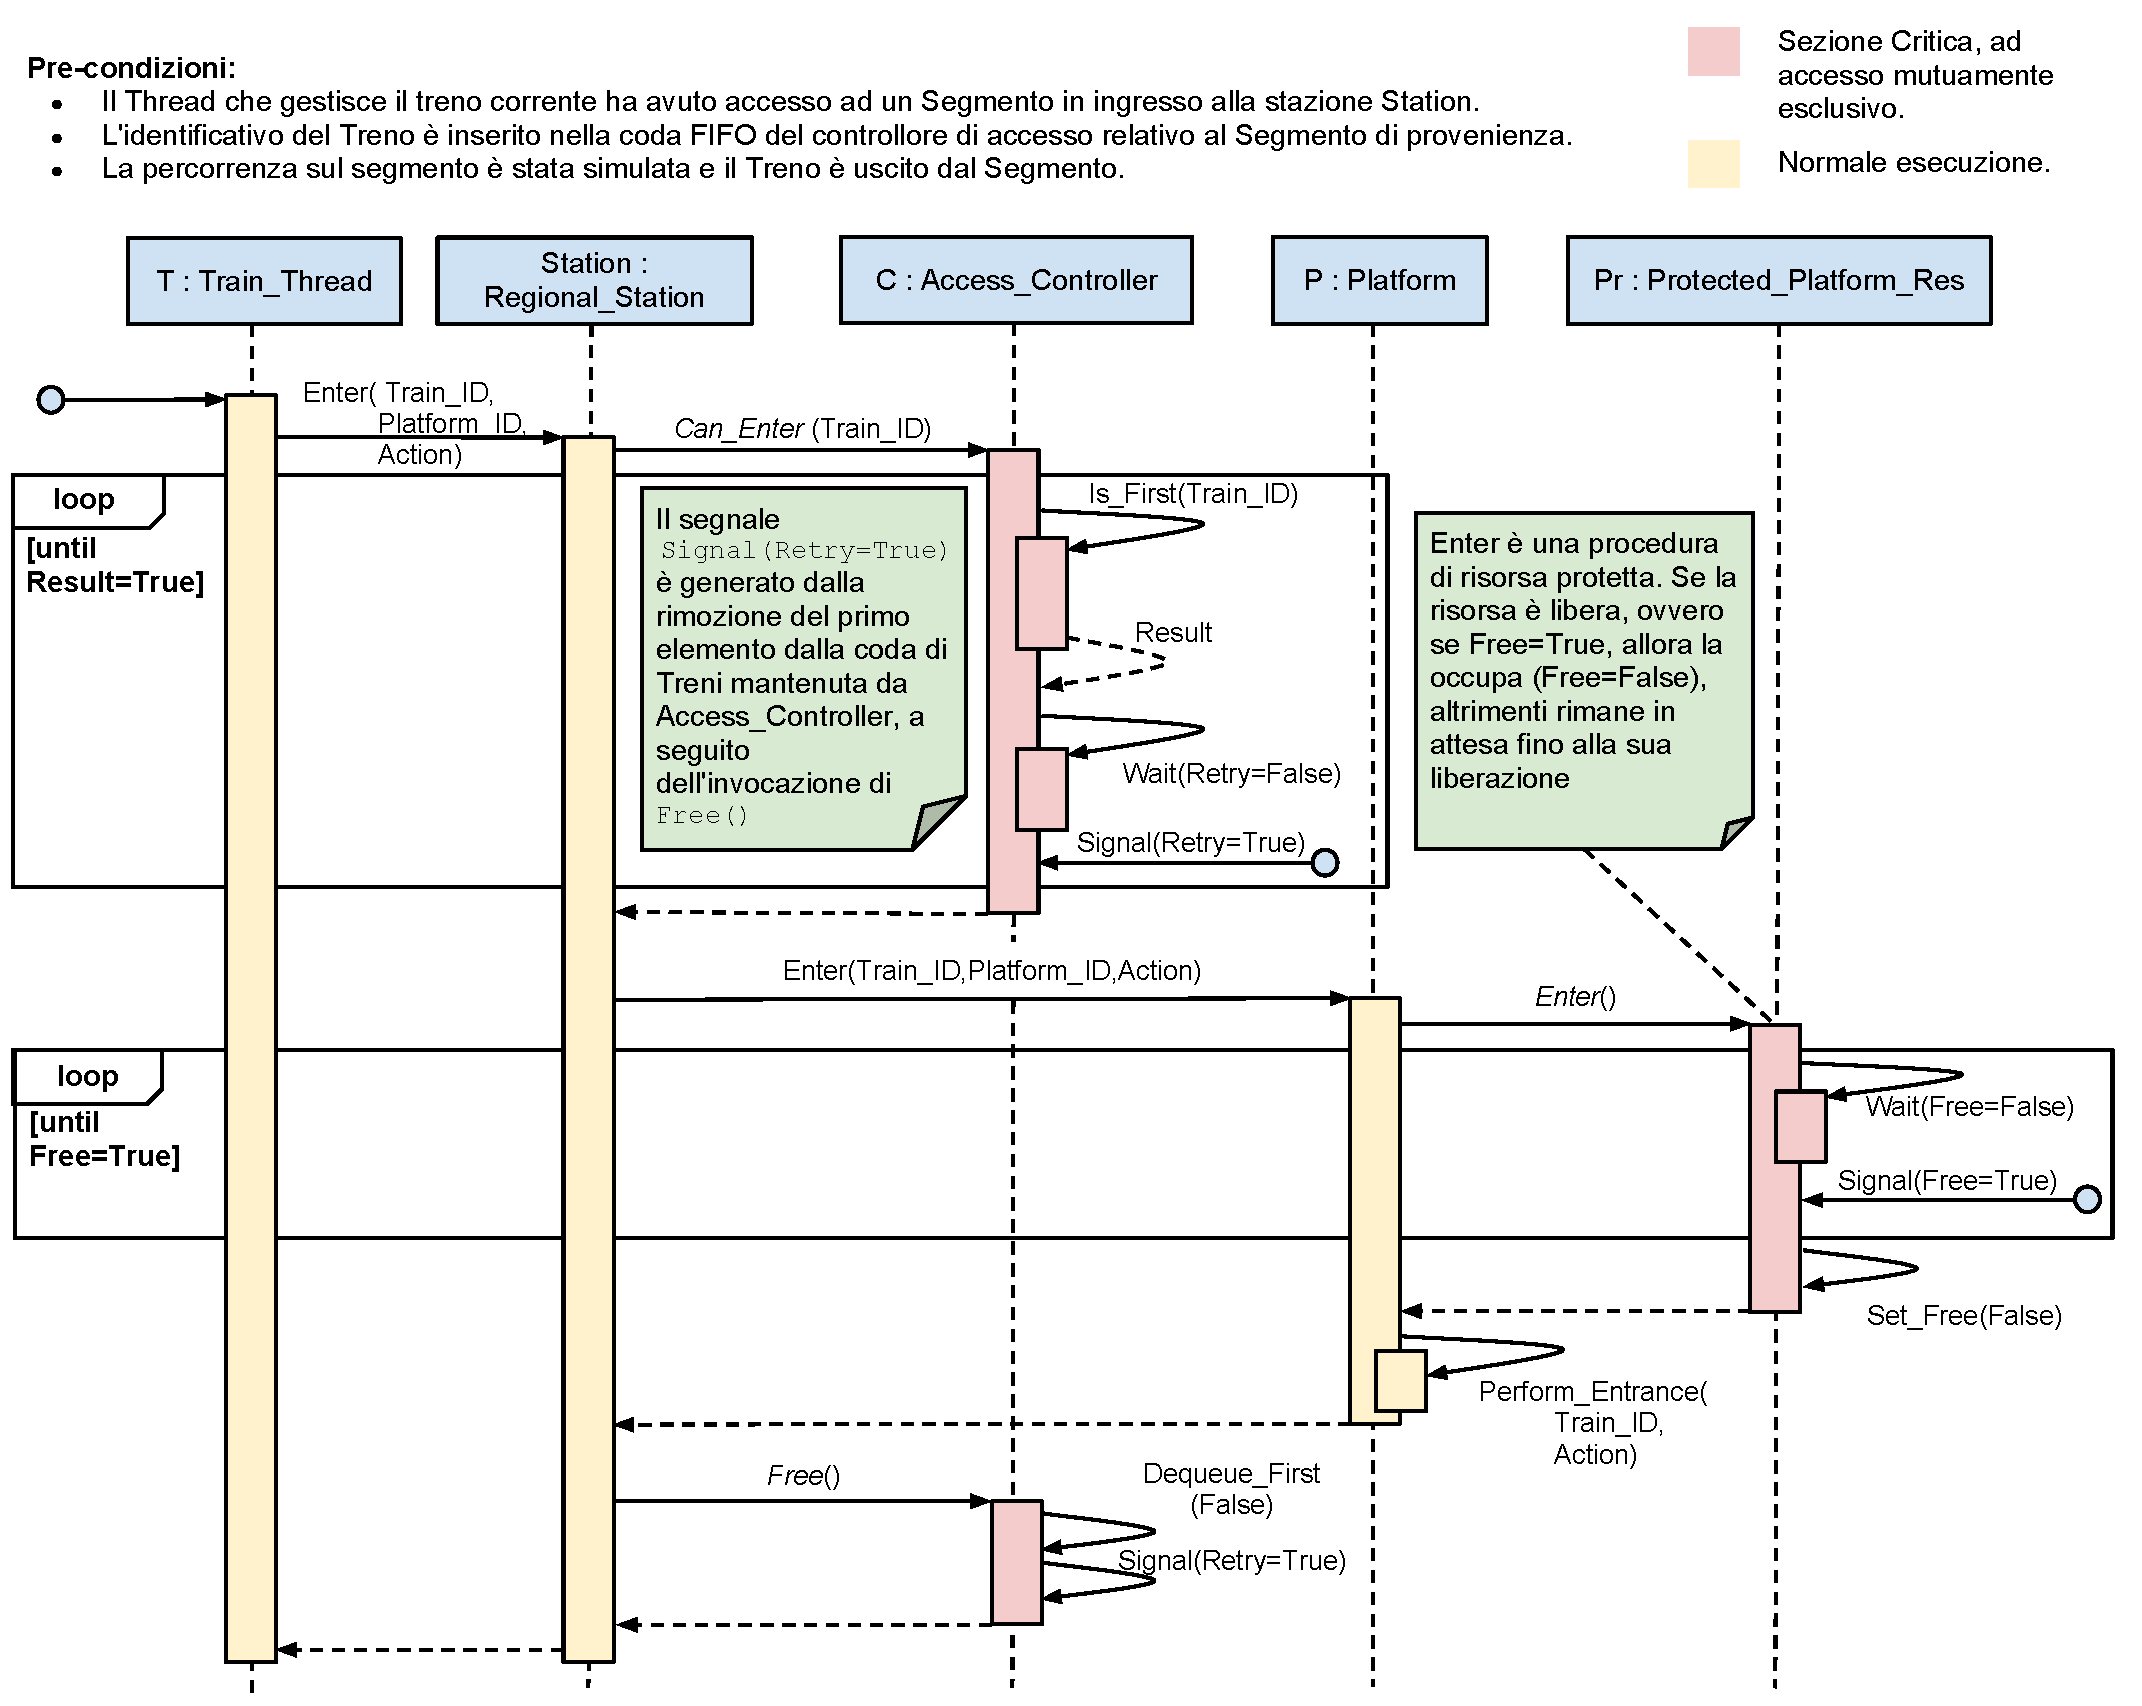
\includegraphics[trim = 55mm 0mm 0mm 0mm,scale=0.53]{imgs/platform_access_Sequence_Diagram.pdf}
			\caption{\footnotesize{Diagramma di Sequenza, operazioni necessarie per l'ingresso in una Piattaforma.}}
			\label{fig:platform_access}
		\end{figure}
		
		I prerequisiti alla richiesta da parte di un Treno $T$ di accesso ad una Stazione sono:
		
			\begin{itemize}
				\item Il Treno $T$ ha avuto accesso ad un Segmento $S$ che collega la stazione corrente a quella dalla quale proviene. Ciò significa che il suo Descrittore sarà stato inserito nella coda \ttt{Train\_Queue} di $S$.
				\item Il Treno $T$ ha simulato la percorrenza su $S$ 
				\item Il Treno $T$ uscito dal Segmento $S$, quindi è stato rimosso dalla coda \ttt{Train\_Queue} di $S$.
			\end{itemize}
			
		Il diagramma di sequenza in figura \ref{fig:platform_access} mostra le operazioni che portano alla richiesta ordinata di accesso, e all'ingresso presso una Piattaforma.
		\begin{description}
	% ################################################# INGRESSO_ORDINATO #########################################
			\item{\ii{Ingresso Ordinato}}
		
		Per tutti i Treni provenienti dallo stesso Segmento, è necessario mantenere un ordine di richiesta di accesso alla Stazione successiva uguale a quello utilizzato per l'uscita dal Segmento. Poiché il sistema non può fare assunzioni sulle politiche di scheduling che saranno adottate, è necessario introdurre un meccanismo che riesca a mantenere l'ordine di richiesta di accesso anche nel caso in cui, il thread che rappresenta il Treno appena uscito dal Segmento venga prerilasciato e venga eseguito il thread rappresentante il Treno successivo.

		Ho vagliato le seguenti soluzioni possibili:
		\begin{enumerate}
			\item Rappresentazione della Stazione come entità passiva ad accesso mutuamente esclusivo. Essa mantiene al suo interno una coda per Segmento, del tutto simile alla coda \ttt{Train\_Queue} interna ai Segmenti, e popolata parallelamente a \ttt{Train\_Queue}. In questo modo è semplice garantire (con un meccanismo simile a quello utilizzato per l'uscita da un Segmento) un accesso ordinato. Questa soluzione ha però uno svantaggio evidente: la richiesta di accesso avviene in mutua esclusione anche tra i Treni provenienti da Segmenti diversi, e che quindi si ritroveranno a dover superare un punto di sincronizzazione inutile, se diretti a Piattaforme diverse della Stazione.
			
			\item Una seconda possibilità prevede la presenza, all'interno di ciascuna Stazione, di una risorsa \ii{monitor} \ttt{Access\_Controller} per ciascun Segmento entrante, la quale si occuperà di garantire l'ordine di accesso mantenendo a tale scopo una coda FIFO interna \ttt{Trains\_Order}. Una volta che il Treno ha guadagnato il permesso di accedere in mutua esclusione alla risorsa protetta di controllo, esso avrà il permesso di interagire con la prossima Piattaforma, in modo concorrente con i Treni provenienti da altri Segmenti entranti. La coda \ttt{Trains\_Order} sarà aggiornata dal Segmento mediante un'invocazione ad una procedura fornita dall'interfaccia della Stazione (ad esempio \ttt{Add\_Train}).
			In questo modo la Stazione diventerà solo un'interfaccia utilizzabile per l'accesso alle piattaforme, e inoltre i vincoli di ordinamento e accesso concorrente alle Piattaforme da Treni provenienti da Segmenti diversi saranno garantiti.
			Un esempio di pseudo-codice per il Controllore di Accessi è riportata nel listato \ref{code:station_access_controller}.
			
\begin{lstlisting}[label=code:station_access_controller,caption=\small{Controllore di Accessi che garantisce accesso ordinato.}]	
monitor Access_Controller
	...
	procedure Add_Train(T:Train)
	begin
		// Accoda il Treno in ingresso nella coda
		// FIFO Trains_Order.
		Trains_Order.Enqueue(T);
	end;

	procedure Enter(T:Train) 
	begin
		// Controlla il primo elemento della coda. 
		// Se coincide con il Treno corrente, il 
		// thread puo' proseguire la propria
		// esecuzione.
		while(T.Id/=Trains_Order.First_Element()) 
		loop
			// Attesa su variabile di condizione, 
			// in attesa di poter ritentare 
			// l'accesso.
			wait(Retry_Enter);
		end loop;
	end;

	procedure Leave()
	begin
		// Risveglia tutti i thread in attesa
		// sulla variabile di condizione
		// Retry_Enter, in modo ordinato. 
		signal_all(Retry_Enter);
	end;
end monitor;
\end{lstlisting}
			
			Lo svantaggio di utilizzare questa soluzione risiede nella creazione delle entità protette, una per ciascun Segmento entrante, che regolano l'accesso ordinato, e quindi spostano parte della conoscenza della topologia della rete ferroviaria anche sulle Stazioni, rendendone più complessa la configurazione iniziale.
			
			\item La terza soluzione esaminata e scelta, è simile alla soluzione precedente, ma a differenza di essa crea una popolazione dinamica di oggetti \ttt{Access\_Controller} che garantiscono l'ordinamento. Ciascun Treno nell'accedere alla Stazione, includerà anche un'identificativo univoco del Segmento di provenienza, e se per esso non esisterà una controllore degli accessi, allora esso verrà creato. Questa variante ha il vantaggio per il quale le stazioni non devono necessariamente essere a conoscenza della topologia del sistema ferroviario; inoltre l'allocazione delle strutture di controllo sarà limitata al massimo al numero di Segmenti in ingresso.
		\end{enumerate} 
		
		Il controllore di accessi (\ttt{Access\_Controller}) ha quindi il compito di far passare solamente il Treno (il thread che lo esegue) che effettivamente è primo nella coda di ordinamento.
		Siano \ttt{Access} e \ttt{Free} rispettivamente le due procedure esposte da \ttt{Access\_Controller}, allora l'accesso alla Piattaforma verrà regolato nel seguente modo:
			\begin{itemize}
				\item Il Treno $T$ usa \ttt{Access} per poter accedere alla prossima Piattaforma.
				\item Se $T$ è effettivamente il primo della Coda allora 
					\begin{itemize}
						\item prosegue con l'accesso alla Piattaforma. 
						\item libera il controllore di accessi \ttt{Access\_Controller} con \ttt{Free}. 
					\end {itemize}
				\item Altrimenti viene messo in attesa del proprio turno su una condizione (\ttt{Retry\_Enter}). I Treni in attesa sulla coda FIFO associata a questa variabile di condizione, verranno risvegliati ogni volta che un Treno effettuerà un accesso e una successiva chiamata a \ttt{Free} (la quale invocherà \ttt{signal(Retry\_Enter)} per ciascun thread in attesa).
			\end{itemize}
		
	% ############################################## INGRESSO_PIATTAFORMA #########################################
		
		\item{\ii{Ingresso in una Piattaforma}}
		
		Dopo aver superato la barriera di controllo d'accesso alla Stazione, rappresentata dalla struttura \ttt{Access\_Controller}, invocando la procedura protetta \ttt{Enter}, ciascun Treno può procedere nel tentativo di ottenere l'accesso alla Piattaforma desiderata. Tale accesso avverrà quindi:
		
		\begin{itemize}
			\item In maniera sequenziale tra tutti i Treni provenienti dallo stesso segmento.
			\item In maniera concorrente tra tutti i Treni provenienti da Segmenti diversi, fornendo precedenza di accesso ai Treni di tipo \ttt{FB}.
		\end{itemize}
		
		Si rende quindi evidente la necessità di garantire l'ordine di esecuzione tra tutti i thread provenienti da uno stesso segmento, indipendentemente dalle politiche di scheduling che verranno adottate. Non è inoltre desiderabile che il thread corrente effettui l'accesso prima di aver rilasciato il controllore di accessi per il Segmento di provenienza. \'E quindi necessario, al rientro della procedura \ttt{Access} del controllore d'accessi, \ii{prenotare} l'accesso alla Piattaforma per poi liberare la risorsa \ttt{Access\_Controller} prima di proseguire con l'ingresso vero e proprio.
				  
		Una Piattaforma è modellata quindi come una struttura dati che contiene una risorsa protetta da \ii{monitor} \ttt{Platform\_Monitor} per la regolazione dell'ordine di ingresso, e che espone un'interfaccia composta da:
		\begin{itemize}
			\item \ttt{Add\_Train}, aggiunge il Descrittore del Treno passato come parametro nella coda FIFO \ttt{Trains\_Access\_Order} della risorsa protetta \ttt{Platform\_Monitor}. Questa coda manterrà l'ordine di accesso alla Piattaforma, non solo tra tutti i Treni provenienti dallo stesso Segmento, ma anche tra i Treni provenienti da Segmenti diversi.
			\item \ttt{Enter\_Platform}, per eseguire l'accesso.
			\item \ttt{Leave\_Platform}, per lasciare la piattaforma.
		\end{itemize}
		Per garantire inoltre che l'ordine di ingresso dei Treni sancito dalla coda \ttt{Trains\_Access\_Order} sia tale da fornire accesso preferenziale ai Treni di tipo \ttt{FB}, viene utilizzato un oggetto \ttt{Priority\_Access\_Handler} come per l'accesso al Segmento (si veda il listato \ref{priority_access_controller}), e di conseguenza il comportamento previsto per la procedura protetta \ttt{Add\_Train} sarà quello riportato nel listato \ref{code:platform_add_train}.
\begin{lstlisting}[caption=\small{Esempio di procedure \ttt{Add\_Train} per l'accesso alla Piattaforma.},label=code:platform_add_train]
	...
	// Procedura Add_Train per l'aggiunta
	// di un descrittore alla coda interna  
	// alla risorsa protetta Platform_Monitor.
	procedure Add_Train(T:Train)
	begin
		Priority_Access.Gain_Access(T);
		// Viene stabilito l'ordine prenotando la 
		// posizione nella coda Trains_Access_Order del
		// monitor a protezione della piattaforma.
		Platform_Monitor.Trains_Access_Order.Enqueue(T);
		Priority_Access.Access_Gained();
	end;
	
\end{lstlisting}
		Una volta aggiunto l'identificativo del Treno corrente in \ttt{Trains\_Access\_Order}, può essere liberata la risorsa di controllo (\ttt{Access\_Controller}) mediante la procedura \ttt{Free} ed è quindi possibile richiedere l'accesso alla Piattaforma successiva prevista dal percorso (l'ordine di ingresso sarà rispettato), che avviene mediante la procedura \ttt{Enter\_Platform} la quale:
		\begin{itemize}
			\item Richiede l'ingresso nella piattaforma tramite la procedura protetta \ttt{Enter\_Monitor} di \ttt{Platform\_Monitor}.
			\item Effettua l'operazione di \bb{Discesa dei Viaggiatori} se previsto dal percorso.
		\end{itemize}
La semantica di accesso ad una Piattaforma $P$ è molto semplice; la procedura di monitor \ttt{Enter\_Monitor} è la seguente:
		\begin{itemize}
			\item Se il Treno corrente $T$ è il prossimo a poter entrare in $P$, allora termina l'esecuzione della procedura.
			\item Se invece $T$ non è il prossimo Treno che può entrare, il Treno viene posto in attesa su variabile di condizione \ttt{Retry\_Enter}.
		\end{itemize}

Si può notare che la struttura dati di controllo per l'accesso ad una Piattaforma è molto simile a quella utilizzata per l'accesso al Segmento (listato \ref{code:station_access_controller}).
		
		L'Operazione di \bb{Discesa dei Viaggiatori}, si basa sulla possibilità che presso la Piattaforma corrente $P$ vi siano Viaggiatori all'interno della coda \ttt{Arrivals\_Queue} in attesa di un evento generato da uno specifico Treno, ovvero il suo arrivo presso $P$. L'operazione di Discesa dei passeggeri ha come precondizione l'accesso alla Piattaforma da parte di un Treno $T$ descritta in precedenza, ed è realizzata dalle seguenti azioni (eseguite dal thread associato a $T$):
		\begin{itemize}
			\item Viene estratto ciascun Viaggiatore $V$ dalla coda \ttt{Arrival\_Queue}, e per ognuno di essi:
			\begin{itemize}
				\item Se il Treno atteso da $V$ (informazione recuperabile dalla Tappa corrente del suo Biglietto) è proprio $T$ allora
					\begin{itemize}
						\item il numero di posti occupati di $T$ viene decrementato;
						\item se la Stazione corrente $S$ \bb{non} è la destinazione che $V$ deve raggiungere allora:
							\begin{itemize}
								\item l'Operazione \ttt{LEAVE} del Viaggiatore viene inserita nella coda di operazioni di \ttt{Traveler\_Pool};
								\item viene incrementato l'indice \ttt{Next\_Stage} nel Biglietto del viaggiatore $V$.
							\end{itemize}
					\end{itemize}
				\item Se $T$ invece non è il Treno atteso da $V$, quest'ultimo viene reinserito nella coda \ttt{Arrivals\_Queue}.
			\end {itemize}
		\end{itemize}
		
	Le operazioni necessarie ad attuare la Discesa dei Viaggiatori devono essere eseguite esternamente alla Sezione critica associata all'ingresso del Treno nella Piattaforma; se così non fosse infatti, essa risulterebbe occupata, e non sarebbe quindi possibile per i thread che sopraggiungono ottenere il blocco esclusivo sulla risorsa per eseguire \ttt{Add\_Train}.
	
	% ################################################# USCITA_PIATTAFORMA #########################################
	\item{\ii{Uscita da una Piattaforma}}

		\begin{figure}[htbp]
			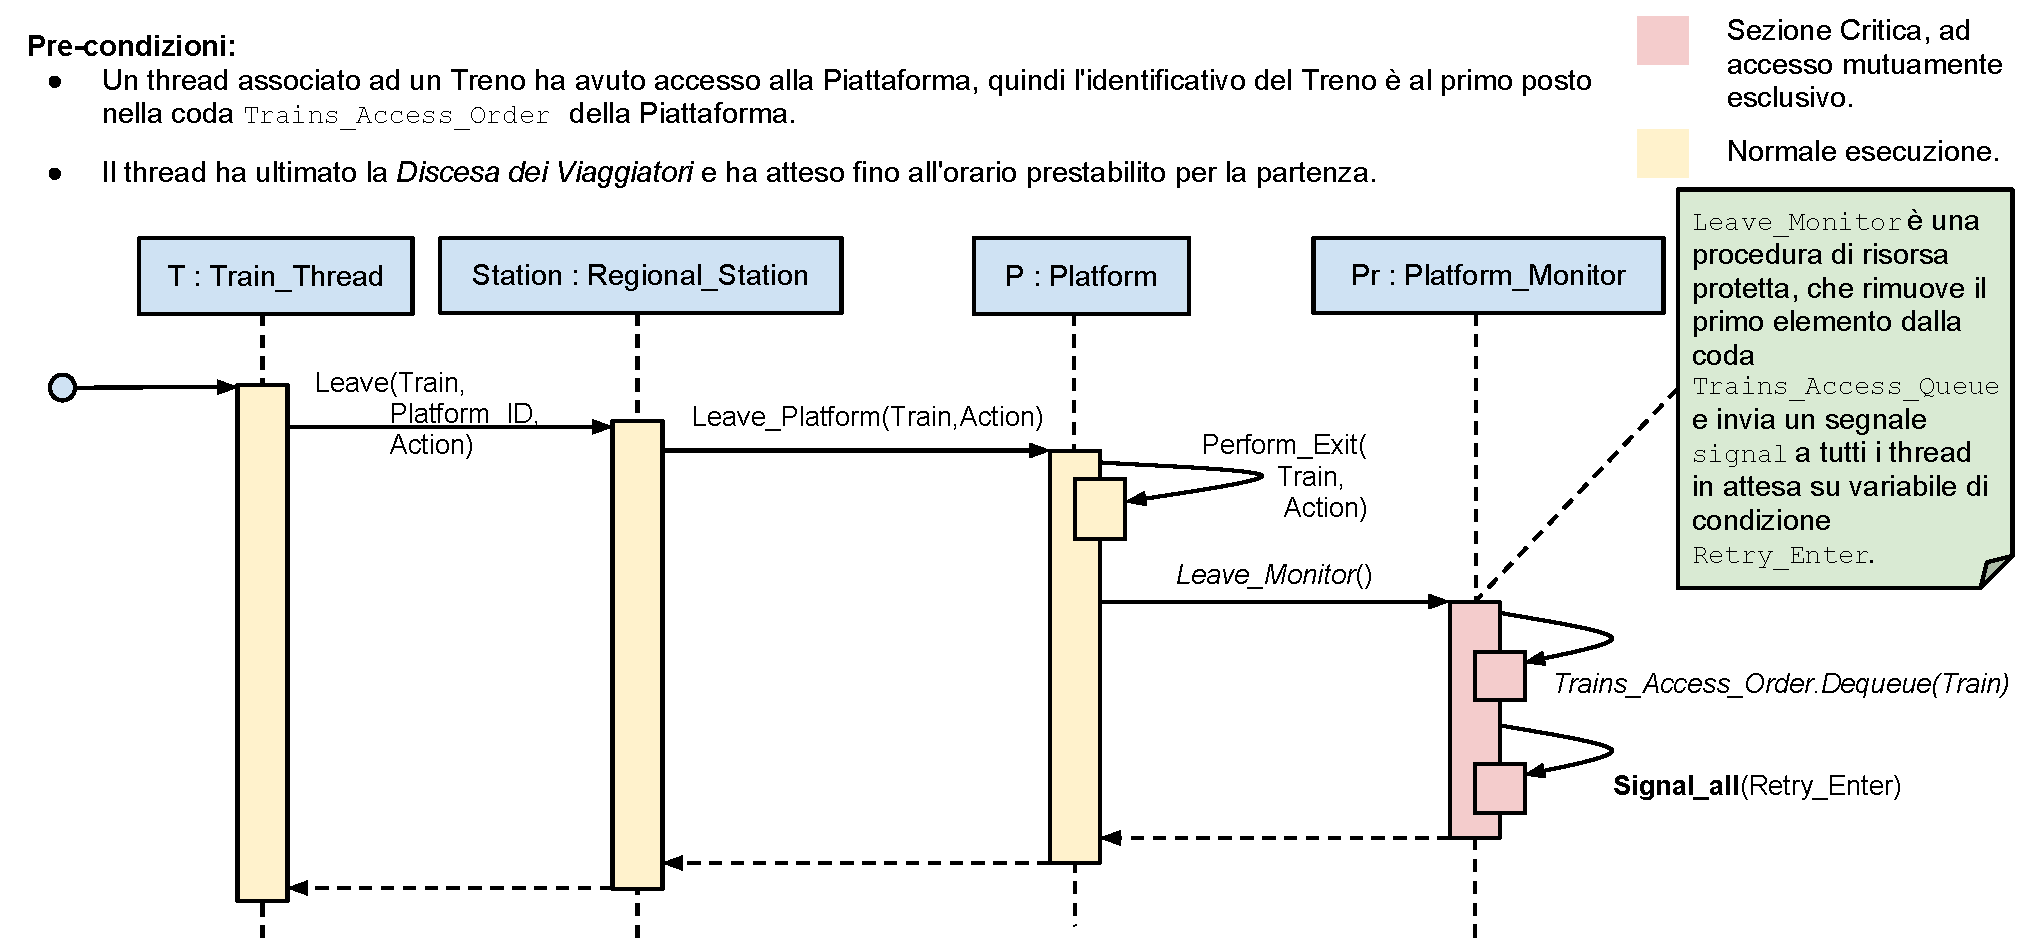
\includegraphics[trim = 45mm 0mm 0mm 0mm,scale=0.55]{imgs/platform_exit_Sequence_Diagram.pdf}
			\caption{\footnotesize{Diagramma di Sequenza, operazioni necessarie per l'uscita da una Piattaforma.}}
			\label{fig:platform_access}
		\end{figure}
		
		L'uscita da una Piattaforma $P$ necessita dei seguenti prerequisiti:
		
			\begin{itemize}
				\item Il thread che gestisce il Treno ha prima effettuato l'ingresso, e quindi il suo identificativo univoco è il primo elemento della coda \ttt{Trains\_Access\_Order} mantenuta dalla risorsa \ttt{Platform\_Monitor} a protezione della Piattaforma.
				\item \'E già stata effettuata la Discesa dei Passeggeri (se prevista dal Percorso del Treno).
				\item \'E stato generato l'evento che notifica al Treno l'arrivo dell'orario previsto per la partenza.
			\end{itemize}
		
		A questo punto, le operazioni effettuate per completare la partenza sono:
		
			\begin{itemize}
				\item Viene effettuata la \bb{Salita dei Viaggiatori} in attesa presso la Piattaforma. 
				\item Il Treno corrente registra il proprio passaggio presso la Piattaforma, memorizzando in una struttura dati apposita \ttt{Last\_Train\_Run} il proprio identificativo univoco e l'identificativo univoco della Corsa corrente \ttt{Current\_Run\_Id}.
				\item La risorsa viene rilasciata dal Treno in esecuzione mediante la procedura di monitor \ttt{Free\_Monitor}, la quale provvede a rimuovere il primo elemento della coda \ttt{Trains\_Access\_Order} e, se ci sono thread in attesa sulla condizione \ttt{Retry\_Enter}, a risvegliare tali thread.
			\end{itemize}
		
		La \bb{Salita dei Viaggiatori} è simile alla discesa dei Passeggeri presentata al punto precedente. Essa prevede l'esecuzione delle seguenti azioni:
		\begin{itemize}
			\item Viene estratto ciascun Viaggiatore $V$ dalla coda \ttt{Leaving\_Queue} di $P$, e per ciascuno di essi:
			\begin{itemize}
				\item Se il Treno atteso da $V$ (informazione recuperabile dalla Tappa corrente del suo Biglietto) è proprio il Treno correntemente in esecuzione $T$ e \ii{se la capienza massima di $T$ non è stata raggiunta} allora:
					\begin{itemize}
						\item il numero di posti occupati di $T$ viene incrementato;
						\item l'Operazione \ttt{ENTER} del Viaggiatore viene \ii{eseguita} a differenza di quanto avviene nella fase di Discesa dei Passeggeri: in questo modo infatti si avrà la garanzia che tutti i Viaggiatori saliti a bordo del Treno saranno in attesa nella coda \ttt{Arrival\_Queue} della Piattaforma di Stazione corretta, nel momento in cui il Treno vi accederà durante il proprio viaggio. 
					\end{itemize}
				\item Se $T$ invece non è il Treno atteso da $V$, allora viene verificato se il Treno per il quale esso è in attesa non sia già passato, qualora esso sia di tipo \ttt{FB}: per effettuare tale controllo viene acceduta la struttura dati \ttt{Last\_Train\_Run} e verificato se la corsa per la quale il Viaggiatore corrente è in attesa del Treno non sia stata già effettuata. In tal caso viene inserita l'operazione \ttt{BUY\_TICKET} per il Viaggiatore corrente nella coda di \ttt{Traveler\_Pool}, per permettere l'acquisto di un nuovo Biglietto per raggiungere la destinazione prevista a partire dalla Stazione corrente. In tutti gli altri casi, il Viaggiatore viene re-inserito nella coda \ttt{Leaving\_Queue}.
			\end {itemize}
		\end{itemize}
	\end {description}

% ############################################################################################################
% ########################################### ACCESSO_STAZIONE_GATEWAY #######################################
% ############################################################################################################		

	\subsubsection{Accesso ad una Stazione di Gateway}\label{subsubsec:gateway_stations_func}
	
	Alcuni Treni seguono percorsi che attraversano più Regioni. Tra le tappe che compongono tali percorsi, alcune indicheranno l'attraversamento di Regioni di Gateway, introdotte nella sezione \ref{sec:gateway_stations}. 
	Le azioni di Ingresso, Salita dei Viaggiatori, e Ripartenza presso questo tipo di stazioni seguono le stesse regole descritte per le stazioni Regionali nella sezione \ref{subsubsec:regional_station_access}. Esse hanno quindi un effetto locale alle Regioni (Nodi) in cui vengono eseguite.
	Per quanto riguarda invece la Discesa dei Viaggiatori, essa può prevedere un \ii{trasferimento remoto} dei Viaggiatori una volta scesi, nel caso essi continuino il proprio viaggio in una Regione diversa.
	
	Il Passaggio di un Treno da una regione alla successiva può essere schematizzato come segue: siano $G1$ e $G2$  Stazioni di Gateway connesse, che collegano le regioni $R1$ ed $R2$, con $G1 \in R1$, e $G2 \in R2$. Un Percorso che attraversa i due Gateway conterrà almeno una Tappa $T1$ tale per cui il campo \ttt{next\_station} avrà il valore $G1$, \ttt{destination\_platform} una delle Piattaforme possibili per effettuare l'accesso $P$, e \ttt{region} la regione $R1$, e una tappa $T2$ tale per cui il campo \ttt{next\_station} avrà il valore $G2$, \ttt{destination\_platform} la stessa piattaforma specificata in $T$, e \ttt{region} la regione $R2$.
	Le operazioni eseguite saranno le seguenti:
	\begin{itemize}
		\item Il Treno corrente $T$ effettua l'accesso alla Stazione $G1$, Piattaforma $P$.
		
		\item $T$, se previsto dal Percorso, effettua Discesa dei Viaggiatori. Tale azione è simile alla Discesa descritta in sezione \ref{subsubsec:regional_station_access}, ma se un Viaggiatore una volta sceso proseguirà il proprio percorso su un nodo diverso da quello corrente, esso verrà trasferito mediante messaggio remoto al nodo successivo (\ii{marshalling} dei dati e invio mediante invocazione remota al Nodo di destinazione), e solo a questo punto verrà inserita l'Operazione \ttt{ENTER} del Viaggiatore nella coda di operazioni di \ttt{Traveler\_Pool} locale al nodo destinazione.
		
		\item Il descrittore del Treno corrente $D_T$ e la sua Tabella degli Orari vengono serializzati (\ii{marshalling}), e inviati tramite invocazione remota al Nodo della Regione $G2$ alla quale appartiene la Stazione di Gateway ad essa connessa. L'individuazione dell'indirizzo della regione specificata nel parametro \ttt{region}, avviene interrogando il \ttt{Name\_Server}, se esso non è già presente in una cache locale.
		\item Il flusso ciclico di istruzioni eseguite dal thread che gestisce $T$ viene interrotto (esso potrà così ottenere un nuovo Descrittore di Treno ed eseguire per esso le proprie operazioni).
		\item Presso la regione $R2$, stazione di Gateway $G2$, vengono eseguite le seguenti operazioni:
			\begin{itemize}
				\item Il Descrittore e la tabella degli orari vengono de-serializzati (\ii{unmarshalling}).
				\item I dati del Descrittore $D_{T'}$ presenti nella regione $R2$ vengono aggiornati con quelli ricevuti. Stessa cosa per la Tabella degli Orari.
				\item Viene aggiunto l'identificativo di $T$ nella coda \ttt{Trains\_Order} della Piattaforma $P$.
				\item Vengono operate attesa fino all'orario di partenza previsto (secondo il clock del nodo corrente), Salita dei Viaggiatori e Partenza dalla Stazione come per le Stazioni Regionali.
				\item Viene restituito un messaggio di \ii{acknowledgement} al nodo $R1$, che comunica l'avvenuta esecuzione delle operazioni.
			\end{itemize}
		\item Una volta ricevuto il messaggio di \ii{acknowledgement}, presso il nodo $R1$, viene liberata la piattaforma corrente (viene rimosso il primo elemento della coda \ttt{Trains\_Order}) in modo tale da permettere ad altri Treni di occuparla.
	\end{itemize}
	
	Ciò che garantisce la correttezza della soluzione presentata, relativamente a discesa e salita dei passeggeri locale, è la modalità con la quale il Viaggiatore viene accodato presso la Stazione di Gateway come descritto nella sezione \ref{subsec:percorrenza_viaggiatore}, ovvero in modo tale per cui:
	\begin{itemize}
		\item Presso le coda \ttt{Arrival\_Queue} delle Piattaforme nel nodo di partenza vi saranno tutti e soli i passeggeri in attesa di scendere presso la Stazione di Gateway, se previsto dal loro Biglietto.
		\item Presso le code \ttt{Leaving\_Queue} delle Piattaforme nel nodo di destinazione vi saranno invece solamente i Viaggiatori che vogliono raggiungere una destinazione interna al nodo corrente.
	\end{itemize}  
	Si noti che la soluzione riportata prevede lo scambio di due messaggi remoti, il primo per la transizione del Treni tra le Regioni, e il secondo di acknowledgement per poter liberare la risorsa Piattaforma presso il nodo di partenza. Di fatto, data l'inaffidabilità della rete, è possibile che uno dei due messaggi scambiati non venga ricevuto dal nodo di destinazione. Abbiamo quindi due casi:
		\begin{itemize}
			\item \ii{L'invio del primo messaggio fallisce.} In questo caso, il flusso di esecuzione del thread che gestisce il Treno viene interrotto. Per semplicità si può pensare che il Treno sia cancellato a causa di un guasto, o si può ridurre il Percorso fino alla Tappa che ha causato l'errore, dopo essersi accertati dell'effettiva irraggiungibilità del nodo destinazione.
			\item \ii{Il messaggio di acknowledgement non viene consegnato.} In questo caso il problema è più grave. Il Treno presso il nodo di destinazione continua la propria corsa, mentre la Piattaforma abbandonata rimane occupata, e quindi inutilizzabile dai Treni che sopraggiungono. Per risolvere questo tipo di problema è possibile prevedere un tempo massimo di occupazione della Piattaforma, oltre il quale richiedere l'effettivo stato di occupazione della Piattaforma presso la Stazione di Gateway della Regione di destinazione e, nel caso in cui risultasse libera, procedere alla liberazione della stessa mediante la procedura \ttt{Leave}.
		\end{itemize}
	 
	

\subsection{Creazione di un Biglietto}

Per la creazione di un Biglietto, necessario per permettere ai Viaggiatori di poter raggiungere una destinazione, ho utilizzato un algoritmo che coinvolge le componenti (distribuite) introdotte in sezione \ref{subsec:ticket_offices}. Per richiedere la creazione di un Biglietto, ho introdotto un tipo di operazione per le entità viaggiatori, che indicherò con \ttt{CREATE\_TICKET}, mentre per gestire l'avvenuta creazione e ottenimento del Biglietto un'operazione che indicherò con \ttt{TICKET\_READY}. Quest'ultima operazione è necessaria poiché l'algoritmo ha una natura asincrona.

La descrizione sarà suddivisa in fasi sucessive:

	\subsubsection {Richiesta di Creazione}
	
	La richiesta di creazione di un \ttt{Ticket} da parte di un Viaggiatore, viene operata da un thread appartenente al pool di \ttt{Traveler\_Pool} che esegue l'operazione \ttt{CREATE\_TICKET}. Tale operazione, effettua una richiesta di creazione alla stazione di partenza $S$, la quale inoltrerà la richiesta alla pripria biglietteria interna. Quest'ultima richiederà la creazione effettiva alla Biglietteria Regionale, se lo stesso \ttt{Ticket} non è presente in una cache locale.  
	
	\subsubsection {Creazione del Ticket}
	
	Siano \ttt{From} e \ttt{To} rispettivamente l'identificativo della Stazione di partenza, e l'identificativo della Stazione di destinazione. Le operazioni svolte dalla procedura invocata presso la Stazione Regionale sono le seguenti:
	\begin{itemize}
		\item Se \ttt{To} appartiene alla Regione corrente, viene creato il \ttt{Ticket}, effettuando le seguenti operazioni:
			\begin {itemize}
					
				\item Si considera il percorso più breve da \ttt{From} a \ttt{To}, che indicheremo con $Path = \{s_1,...,s_N\}$. Questo percorso è ottenuto applicando un semplice algoritmo di cammino minimo sul grafo avente come veritici le Stazioni, e come archi non direzionati i Segmenti che li collegano. Il cammino può minimizzare la lunghezza totale del percorso.
				
				\item Il percorso $Path$ viene intersecato con i Percorsi dei Treni (\ttt{Route}), per poter definire le Tappe che compongono il Biglietto. Sia $i=1$, allora finché $i<=N$:
					\begin{itemize}
						\item Ottieni i percorsi dei Treni (\ttt{Route}s) $R={r_1,...,r_k}$ che contengono una Tappa $t$ tale per cui i campi \ttt{Start\_Station} e \ttt{Next\_Station} sono rispettivamente $s_i$ e $s_{i+1}$. Per ciascuno di questi percorsi, vengono ottenuti indice e posizione della tappa $t$ al suo interni.
						A qusto punto si procede all'individuazione del percorso che meglio si adatta al cammino minimo da segire. Sia quindi $k = i$; per ciascuna route $r_j \in R$, a partire dalla posizione di $t$ in $r_j$, si procede ad estendere la corrispondenza. Viene quindi mantenuto il percorso con la corrispondenza di lunghezza massima $Max\_Length$, memorizzandone l'indice in $Max\_Match$.
						\item Viene quindi creata una Tappa del \ttt{Ticket}:
						\begin{verbatim}
							- start_station        : indice della stazione 
							                         di inizio dell'estensione,
							- next_station         : indice della stazione di
							                         fine dell'estensione 
							                         massima,
							- train_id             : indice del Treno che 
							                         percorre il percorso di 
							                         indice Max_Match,
							- start_platform       : indice della Piattaforma
							                         di partenza in t,
							- destination_platform : indice della Piattaforma 
							                         dell'ultima tappa
							- next_region          : regione corrente,
							
						\end{verbatim}
						\item $i$ viene incrementato di $Max\_Length$.
					\end{itemize} 
			\item Il \ttt{Ticket} creato viene assegnato al Viaggiatore e viene quindi inserita l'operazione \ttt{TICKET\_READY} nella coda di operazioni di \ttt{Traveler\_Pool}.
			\end {itemize} 
		\item Se \ttt{To} non appartiene alla Regione corrente, allora viene effettuata una richiesta remota alla Biglietteria Centrale. Tale richiesta è asincrona, in modo tale da permettere al thread che sta effettuando la richiesta di creazione del Biglietto di non effettuare attesa attiva, e quindi di poter eseguire altre operazioni eventualmente presenti nella coda di \ttt{Traveler\_Pool}.
	\end{itemize} 
	
	\subsubsection {Richiesta di Creazione Remota}
	
	Una volta che la Biglietteria Centrale riceve, tramite l'interfaccia remota esposta, un messaggio remoto di richiesta di Creazione di un Biglietto, essa effettua 3 operazioni:
	\begin{itemize}
		\item Individua la Regione di appartenenza della destinazione $To$; se tale informazione non è presente nella cache locale mantenuta dalla Biglietteria Centrale, essa viene ricercata nel modo seguente: 
			\begin{itemize}
				\item viene recuperato l'elenco completo delle Regioni (ovvero una lista di coppie \ttt{(Node\_Name,Node\_Address)}) dal \ii{Server dei Nomi};
				\item per ciascun elemento dell'elenco, viene inviata una richiesta remota, alla quale ciascuna Regione risponde con \ttt{True}, se contiene la Stazione, o \ttt{False} in caso contrario.
			\end{itemize}
		\item Se nessuna risposta positiva viene ricevuta, allora viene comunicato l'errore alla Biglietteria Regionale richiedente, inviando un messaggio di errore.
		\item Nel caso in cui si abbia una risposta positiva da una Regione $R$ allora:
			\begin{itemize}
				\item Viene recuperata la lista di Regioni attraverso le quali costruire il percorso per raggiungere la destinazione (dalla mappa \ttt{Links}). 
				\item A ciascuna stazione di questa lista viene inviata una richiesta remota \ii{sincrona} per ottenere dei Ticket che collegati, permettono di raggiungere \ttt{To} a partire da \ttt{From}.
				\item I vari \ttt{Ticket} ottenuti vengono poi uniti (eliminati i passaggi per le stazioni di gateway se non necessari) e il Biglietto risultante inviato come risposta al Nodo richiedente, presso il quale verrà assegnato al viaggiatore richiedente, e verrà inserita l'operazione \ttt{TICKET\_READY} nella coda di \ttt{Traveler\_Pool}.
			\end{itemize}
	\end{itemize}

\subsection{Terminazione distribuita}\label{sec:distributed_termination}


